
\section{Project Management and Industry Collaborations}
%
%Please refer to the supplemental document titled Collaboration
%Plan.

The research team poses complementary skills required for the
project. The PIs are well qualified for the proposed research with
significant prior experience in various areas. The PI Prof. Li has
5-years industrial experience related to device modeling and circuit design with focus
on emerging non-volatile memories, and just recently joined NYU-Poly as
an assistant professor. The co-PI Prof. Xie's
expertise span areas of VLSI and architecture, with extensive experience
in architectures with emerging technologies, such as 3D architecture.
The PIs will work in close coordination on
different parts of this project. The
integration of all these research components and tool will be a
coordinated effort by all the investigators. The project is a three-year
effort involving multiple PhD students. Li will lead the effort in
the first year with 2 PhD students from NYU working with 1 PhD student
from PSU on the circuit and architectural modeling in Task 1. In the second
year, Xie will lead the effort in Task 2, with 2 PhD students from PSU and
1 student from NYU, to study architectural techniques using NVM technologies. In the final year, both PIs will work together with 1 PhD from each institute to study novel applications that leverage NVM technologies.
Detailed project milestones are given in Figure~\ref{fig:plan}.

%\begin{comment}
%\begin{wrapfigure}{r}{0.5\textwidth}
%\vspace{-10pt}
\begin{figure}[htp]
\centering
% Requires \usepackage{graphicx}
%\epsfig{file=./figure/3DTESTDFT1.eps,width=0.5\textwidth}
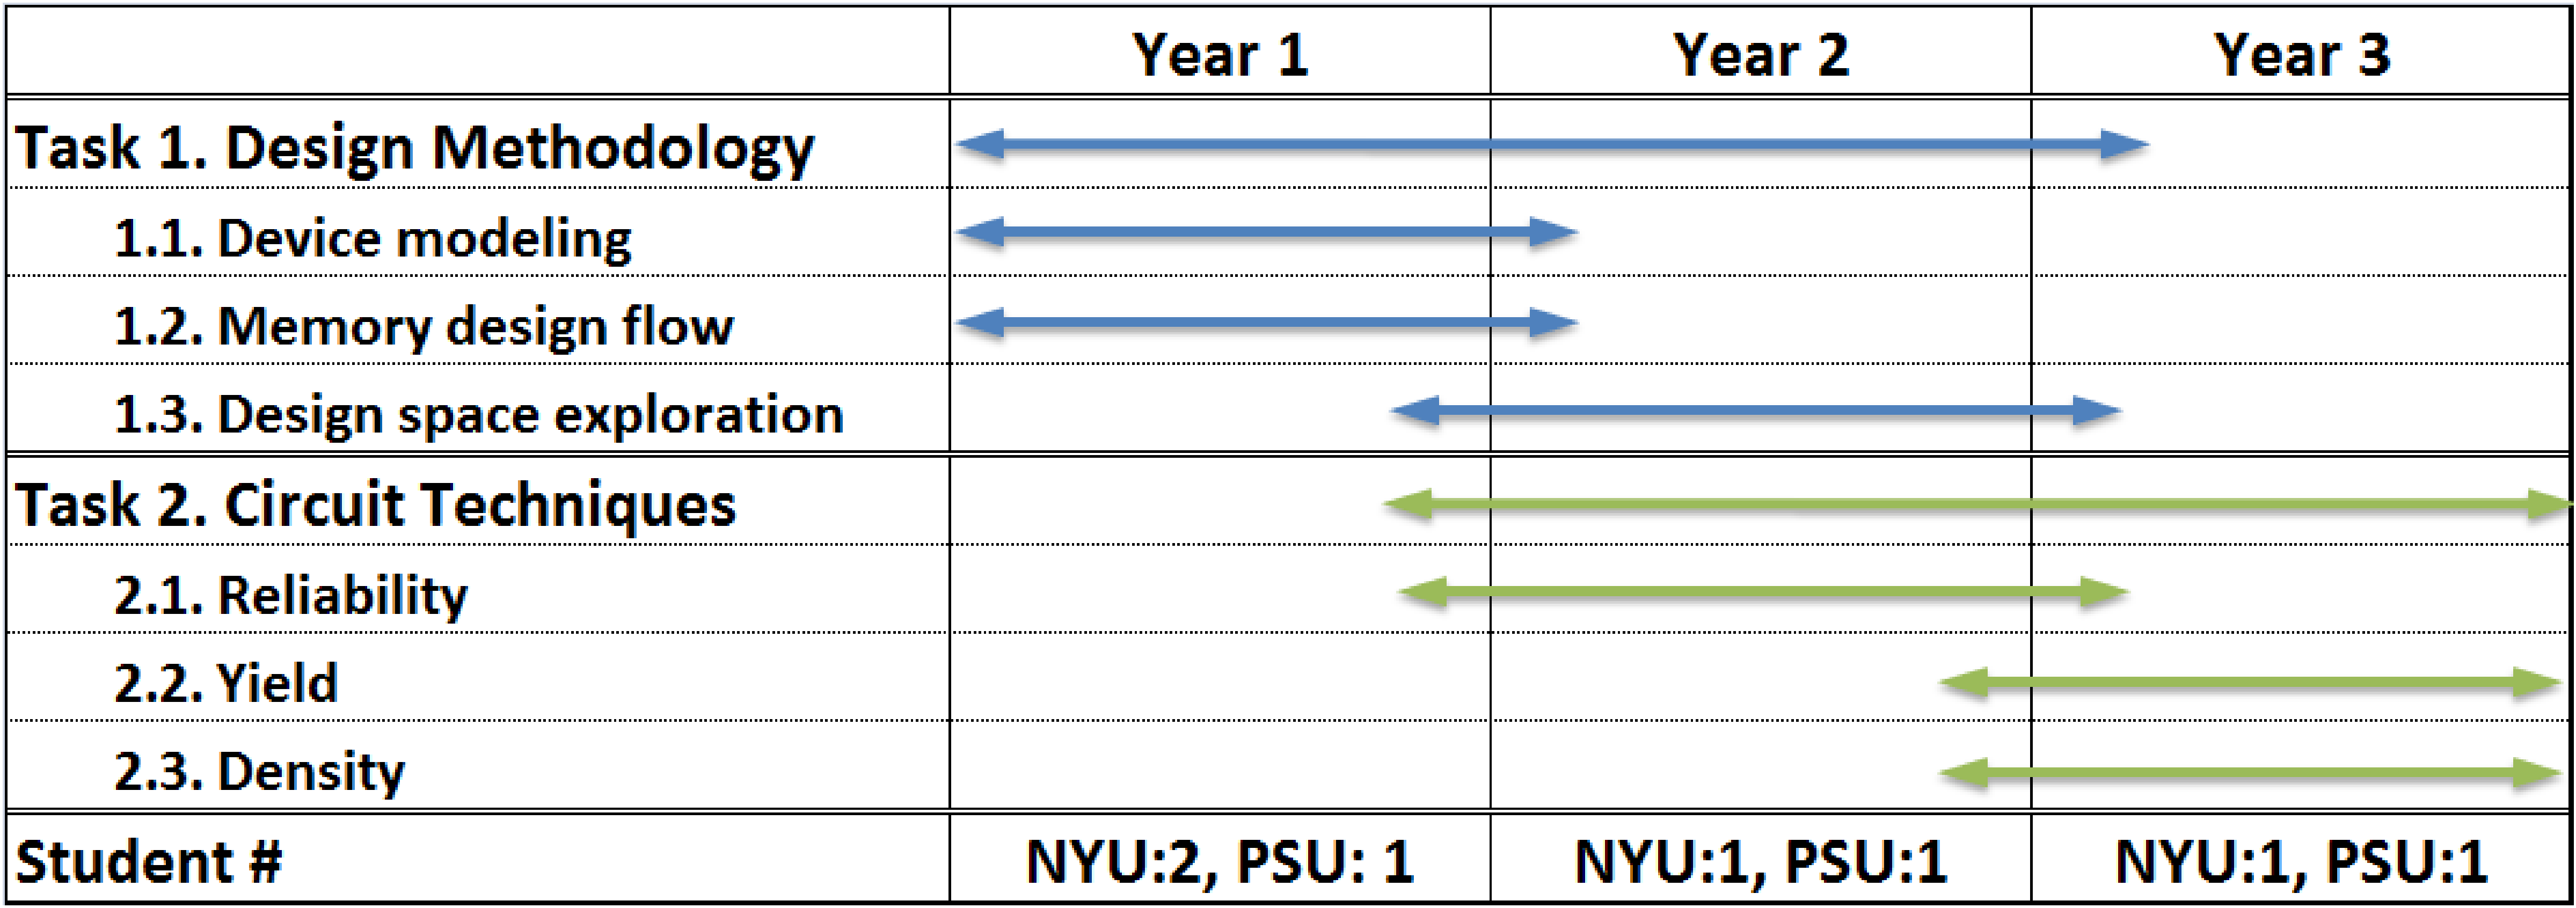
\includegraphics[width=0.6\textwidth]{./figure/schedule.pdf}
\vspace{-10pt} \caption{Project Management (The first
student in each task would be the lead).}\label{fig:plan}
\end{figure}
%\vspace{-10pt}
%\end{wrapfigure}
%\end{comment}


The PIs have a well-established collaboration in the past years,
when the PI was still in Seagate,  and published preliminary results
on NVM architectures in DAC 2008 and HPCA 2009~\cite{XIE:HPCA09,Xie:dac08}. The existing collaboration
and preliminary results will allow rapid ramp-up for the proposed
research. The two teams will coordinate with each other via weekly
teleconferences and regular mutual visits (with only 4-hour driving between
two institutes).

\paragraph{\textbf{Industry Collaborations.}} By leveraging both PI's past industry experience and successful collaborations with companies, the project will be carried out in close collaboration with
industrial partners from IBM, HP, Intel, Qualcomm, Seagate, ITRI, as well as with
a partner from IMEC in Belgium. 
The industrial collaborators will play important roles in the
proposed project by enabling the acquisition of realistic data,
discussion of the practicality of ideas, placement of students in
internships and permanent positions, and eventually the transfer of
the technologies. By working closely with researchers in industry,
the PIs will be able to ensure that the proposed methodologies and
tools are practical and have a real impact on industry.


\section{Results
from Prior NSF Support} \label{sec:prior}

\paragraph{Hai (Helen) Li} recently just joined NYU-Poly as an assistant
professor, after 5-years industrial experience in Qualcomm, Intel,
 and Seagate. She doesn't have any NSF grant yet.

\paragraph{\textbf{Yuan Xie:}} The most related prior NSF grant is
CCF-0903432 (ADAM: Architecture and Design Automation for 3D
Multi-core Systems; 08/2009-07/2012; \$480K). This project aims at
developing architectural design techniques and design automation
tools for future 3D multi-core architectures.
Xie actively collaborates with industry in 3D IC design research
(IBM, Qualcomm, Honda, and Seagate). He has published extensively in
the 3D IC design and 3D architecture areas, covering various aspects, including 3D
architecture~\cite{Xie:MTDT09,XIE:ASPDAC09-3D,XIE:HPCA09,Xie:dac08,xie:isca08,Xie:ISCA09,xie:isca06,xie:iccd05-3d,3D:LXB07,xie:tutorial-micro06} and
3D EDA
tools~\cite{XIE:ASPDAC2009-3Dcost,xie:iccd07-3d,XIE:ICCD08-3D,xie:isqed06-3d,xie:aspdac06,XIE:TVLSI2008-3DCacti,xie:iccd05-3d,xie:jetcs06}.

One of the benefits for 3D integration technologies is
the capability of enabling cost-effective heterogeneous integration, which
makes it much more practical to integrate emerging NVM with CMOS logic circuits.
Consequently, the research plan described in this proposal will
complement and be synergistic with the ongoing project.

The PIs have also submitted another proposal titled "Collaborative Research:SHF:Small:Modeling, Architecture and Application for Emerging Memory Technologies`` to NSF-CISE-CCF-SHF program recently (December 2009), with a focused
scope of computer architecture research. The research topics work proposed in this proposal is circuit-oriented, and will complement and be synergistic with the other
pending proposal.

 \begin{comment}
\paragraph{Yuan Xie} has been awarded 7 NSF grants since 2003: 1) NSF
CNS 0454123:
 {\em SEAT -- Soft Error Analysis Toolset }(co-PI).
  06/2005-05/2008. This CRI (Computer Research Infrastructure)
  project aims at developing a soft error
  analysis toolset for hardware.
  Some of the results have been published
  \cite{xie:vlsid06-raj,
  xie:isvlsi06-soc,xie:selse06-raj,xie:selse06-balaji,xie:selse06-wang,
  xie:vlsid07-ser, xie:date07-timing, xie:date07-nbti, xie:isqed07-ser}.
2)NSF CAREER {\em CNS-0643902: Process Variation Aware Embedded
System Synthesis}.01/2007-12/2011. This CAREER project aims at
developing variation aware analysis and synthesis techniques for
embedded system design. The project has resulted in a few
publications~\cite{xie:date07-nbti,xie:date07-timing,xie:iccad07},
including ASP-DAC 2008 Best Paper Award
Nomination~\cite{xie:aspdac08}. 3)(NSF): {\em CCF 0702617: HoDoo:
Holistic Design of On-chip Interconnects}. 08/2007-07/2010. This
project aims at developing high performance, low power, reliable
on-chip network for future NoC architectures. 4)NSF {\em CNS
0720659: Hybrid Timing Analysis via Multi-mode Execution}.
01/2008-12/2010. This project aims at developing worst-case
execution time analysis techniques for embedded systems that
employ modern microarchitectures. He has been recently awarded 3
new NSF grants, which are all starting from 08/2009. These 3
grants include: 1) NSF 0903432. ``ADAM: Architecture and Design
Automation for 3D Multi-core Systems" (PI), 08/2009-07/2012. 2)NSF
0905365: ``Providing Predictable Timing for Task Migration in
Embedded Multi-Core Environments (TiME-ME)" (PI), 08/2009-07/2013.
3)NSF 0916887: ``Improving Lifetime Reliability for Reconfigurable
Embedded Systems" (Co-PI), 08/2009-07/2012.
\end{comment}

